\documentclass[9pt,twocolumn,twoside]{../../styles/osajnl}
\usepackage{fancyvrb}
\journal{i524} 

\title{Facebook Tao}

\author[1,*]{Nandita Sathe}

\affil[1]{School of Informatics and Computing, Bloomington, IN 47408, U.S.A.}

\affil[*]{Corresponding author: nsathe@iu.edu}

\dates{paper-2, \today}

\ociscodes{Facebook Tao, Graph Database, memcache}

% replace this with your url in github/gitlab
\doi{\url{https://github.com/nsathe/sp17-i524/blob/master/paper2/S17-IO-3017/report.pdf}}


\begin{abstract}
As early as 2005, Facebook started using MySQL, a relational database coupled with large distributed cache called memcache. Facebook soon realized however efficient relational database it would use, it is not sufficient to manage the enormous data challenge Facebook had. The data was a social graph. Another mismatch, which relational database or block cache had was, most of the data that would be read into cache did not belong to any relation. For example, 'If user likes that picture". In most records the answer would be 'No' or 'False'. Storing and reading this unwanted data was a burden. Meanwhile Facebook users' base was increasing daily. Ultimately Facebook came up with Facebook Tao, a distributed social graph data store.  
\newline
\end{abstract}

\setboolean{displaycopyright}{true}

\begin{document}

\maketitle

\section{Introduction}

In the paper published in USENIX annual technical conference, Facebook Inc describes TAO (The Association and Objects) as \cite{book-tao1} a geographically distributed data store that provides timely access to the social graph for Facebook’s demanding workload using a fixed set of queries. It is deployed at Facebook for many data types that fit its model. The system runs on thousands of machines, is widely distributed, and provides access to many petabytes of data. TAO represents social data items as Objects (user) and relationship between them as Associations (liked by, friend of). TAO cleanly separates the caching tiers from the persistent data store allowing each of them to be scaled independently. To any user of the system it presents a single unified API that makes the entire system appear like 1 giant graph database \cite{www-tao1}.
Key advantages of the system include \cite{www-tao1}:
\begin{itemize}
\item Provides a clean separation of application/product logic from data access by providing a simple yet powerful graph API and data model to store and fetch data. This enables Facebook product engineers to move fast.
\item By implementing a write-through cache TAO allows Facebook to provide a better user experience and preserve the all important read-what-you-write consistency semantics even when the architecture spans multiple geographical regions.
\item By implementing a read-through write-through cache TAO also protects the underlying persistent stores better by avoiding issues like thundering herds without compromising data consistency.

\end{itemize}

\section{Tao's Goal}
Main goal of implementing Tao is efficiently scaling the data. Facebook handles approximately a billion requests per second. So obviously data store has to be scalable. More than that, scalability should be efficient otherwise scaling data across machines would be extremely costly. 

Second goal is to achieve lowest possible read latency. So that if a user has commented on a post, the original post writer should be able to read it immediately.
Efficiency in Scaling and low Read latency is achieved by (i) separating cache and data storage, (ii) Graph specific caching and (iii) Sub-dividing data centers \cite{www-tao4}.

Third goal is to achieve timeliness of writes. If a web server has written something and it sends a read request, it should be able to read the post. Write timeliness is achieved by (i) Write trough cache and (ii) Asynchronous replication \cite{www-tao4}.

Lastly high read availability for the same reasons mentioned above, which is achieved by using alternate data sources.

\section{Tao Data Model and API}
Facebook Inc. explains TAO data model and API associated with using a simple example \cite{www-tao2}. Figure \ref{fig:figure1} depicts TAO data model.

\begin{figure}[htbp]
\centering
\fbox{\includegraphics[width=\linewidth]{images/TAOdatamodel.eps}}
\caption{TAO Data Model \cite{www-tao2}.}
\label{fig:figure1}
\end{figure}

This simple example shows a subgraph of objects and associations that is created in TAO after Alice checks in at the Golden Gate Bridge and tags Bob there, while Cathy comments on the check-in and David likes it. Every data item, such as a user, check-in, or comment, is represented by a typed object containing a dictionary of named fields. Relationships between objects, such as “liked by" or “friend of," are represented by typed edges (associations) grouped in association lists by their origin. Multiple associations may connect the same pair of objects as long as the types of all those associations are distinct. Together objects and associations form a labeled directed multigraph.

For every association type a so-called inverse type can be specified. Whenever an edge of the direct type is created or deleted between objects with unique IDs id1 and id2, TAO will automatically create or delete an edge of the corresponding inverse type in the opposite direction (id2 to id1). The intent is to help the application programmer maintain referential integrity for relationships that are naturally mutual, like friendship, or where support for graph traversal in both directions is performance critical, as for example in “likes” and “liked by."

\subsection{Objects and Associations}
\cite{book-tao1} TAO objects are typed nodes, and TAO associations are typed directed edges between objects. Objects are identified by a 64-bit integer (id) that is unique across all objects, regardless of object type (otype). Associations are identified by the source object (id1), association type (atype) and destination object (id2). At most one association of a given type can exist between any two objects. Both objects and associations may contain data as key→value pairs. A per-type schema lists the possible keys, the value type, and a default value. Each association has a 32-bit time field, which plays a central
role in queries.

Object: (id) -> (otype, (key -> value)∗)

Assoc.: (id1, atype, id2) -> (time, (key -> value)∗)

Figure 1 shows how TAO objects and associations might encode the example, with some data and times omitted for clarity. The example’s users are represented by objects, as are the checkin, the landmark, and Cathy’s comment. Associations capture the users’ friendships, authorship of the checkin and comment, and the binding between the checkin and its location and comments.

The set of operations on objects is of the fairly common create/set-fields/get/delete variety. All objects of a given type have the same set of fields. New fields can be registered for an object type at any time and existing fields can be marked deprecated by editing that type’s schema. In most cases product engineers can change the schema of their types without any operational work.

Associations are created and deleted as individual edges. If the association type has an inverse type defined, an inverse edge is created automatically. The API helps the data store exploit the creation-time locality of workload by requiring every association to have a special time attribute that is commonly used to represent the creation time of association. TAO uses the association time value to optimize the working set in cache and to improve hit rate.

There are three main classes of read operations on associations \cite{www-tao2}:
\begin{itemize}

\item Point queries look up specific associations identified by their (id1, type, id2) triplets. Most often they are used to check if two objects are connected by an association or not, or to fetch data for an association. 
\item Range queries find outgoing associations given an (id1, type) pair. Associations are ordered by time, so these queries are commonly used to answer questions like "What are the 50 most recent comments on this piece of content?" Cursor-based iteration is provided as well.
\item Count queries give the total number of outgoing associations for an (id1, type) pair. TAO optionally keeps track of counts as association lists grow and shrink, and can report them in constant time
\end{itemize}

\section{TAO Architecture}

This section describes the architecture of TAO. TAO is separated into layers: two caching layers and a storage layer.
\subsection{Storage Layer}

The data is persisted using MySQL. The API is mapped to a small number of SQL queries. Data is divided into logical shards. By default all object types are stored in one table and association in others. Every 'object-id' has a corresponding 'shard-id'. Objects are bounded to a single shard throughout their lifetime. An association is stored on the shard of its id1, so that every association query can be served from a single server \cite{www-tao4}.

\subsection{Caching Layer}
TAO’s cache implements the complete API for clients, handling all communication with databases. A region/tier is made of multiple closely located Data centers. Multiple Cache Serves make up a tier (set of databases in a region are also called a tier) that can collectively capable of answering any TAO Request. Each cache request maps to a server based on sharding. The cache is filled based on a LRU policy. Write operations on an association with an inverse may involve two shards, since the forward edge is stored on the shard for id1 and the inverse edge is on the shard for id2. Handling writes with multiple shards involve: Issuing an RPC call to the member hosting id2, which will contact the database to create the inverse association. Once the inverse write is complete, the caching server issues a write to the database for id1. TAO does not provide atomicity between the two updates. If a failure occurs the forward may exist without an inverse, these hanging associations are scheduled for repair by an asynchronous job \cite{www-tao4}.

\subsection {Leaders and Followers}
There are two tiers of caching clusters in each geographical region. Clients talk to the first tier, called followers. If a cache miss occurs on the follower, the follower attempts to fill its cache from a second tier, called a leader. Leaders talk directly to a MySQL cluster in that region. All TAO writes go through followers to leaders. Caches are updated as the reply to a successful write propagates back down the chain of clusters. Leaders are responsible for maintaining cache consistency within a region. They also act as secondary caches, with an option to cache objects and associations in Flash \cite{www-tao2}.

\subsection {Scaling Geographically}
High read workload scales with total number of follower servers. The assumption is that latency between followers and leaders is low. Followers behave identically in all regions, forwarding read misses and writes to the local region’s leader tier. Leaders query the local region’s database regardless of whether it is the master or slave. This means that read latency is independent of inter-region latency. Writes are forwarded by the local leader to the leader that is in the region with the master database. Read misses by followers are 25X as frequent as writes in the workload thus read misses are served locally. Facebook chooses data center locations that are clustered into only a few regions, where the intra-region latency is small (typically less than 1 millisecond). It is then sufficient to store one complete copy of the social graph per region.

Since each cache hosts multiple shards, a server may be both a master and a slave at the same time. It is preferred to locate all of the master databases in a single region. When an inverse association is mastered in a different region, TAO must traverse an extra inter-region link to forward the inverse write. TAO embeds invalidation and refill messages in the database replication stream. These messages are delivered in a region immediately after a transaction has been replicated to a slave database. Delivering such messages earlier would create cache inconsistencies, as reading from the local database would provide stale data. If a forwarded write is successful then the local leader will update its cache with the fresh value, even though the local slave database probably has not yet been updated by the asynchronous replication stream. In this case followers will receive two invalidates or refills from the write, one that is sent when the write succeeds and one that is sent when the write’s transaction is replicated to the local slave database \cite{www-tao4}.

\section{Educational Material}

To get started on learning Facebook TAO, following resources can prove helpful.

\begin{itemize}
\item \cite{book-tao1} - Technical paper on Facebook TAO.

\item \cite{www-tao2} - Background, Architecture and Implementation from Facebook itself.

\item \cite{www-tao3} - TAO summary in a video on USENIX website.

\end{itemize}

\section {Acknowledgements}
The author would like to thank Prof. Gregor von Laszewski and his associates from the School of Informatics and Computing for providing all the technical support and assistance.

% Bibliography

\bibliography{references}
\end{document}
